\section{Intelligent Agents}
\textbf{Professor's slides}:\newline
\url{../other/professor's slides/Part III - Intelligent agents.pdf}
\subsection{Agent-Environment interaction}
What is an agent? Intuitively, an \textbf{agent} is a system that is able to \textbf{act}.\newline
\newline
In general, an agent performs an action on its \textbf{environment}: therefore, what we call
an action is actually an \textbf{agent-environment interaction}. To give a more general idea of what an agent is, we shall first consider agents that have
both a “mind” and a “body” (biological organisms, robots); a pure software agent can then
be viewed as a special case, in which there is no “body” properly so called.\newline
\newline
The interaction between an agent and its environment consists of two \textbf{streams of} physical
\textbf{events}, one in \textbf{input} to the agent, the other one in \textbf{output}.\newline
\newline
The function of an agent is to \textbf{control its environment}, in order to achieve certain \textbf{goals}.\newline
\newline
At the interface with its environment, an agent has to:
\begin{itemize}
    \item transform the input physical events into input data suitable for internal processing performed by what we can call the agent’s \textbf{controller};
    \item tranform the output data of internal processing into the output physical events.
\end{itemize}
These operations are performed by two types of devices, called \textbf{transducers}:
\begin{itemize}
    \item input transducers, called \textbf{sensors};
    \item output transducers, called \textbf{actuators} or effectors.
\end{itemize}
\begin{center}
    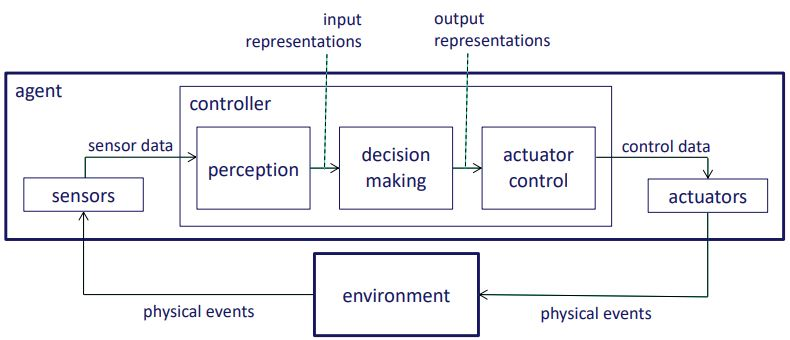
\includegraphics[height=6cm]{../arguments/SensorsAndActuators.JPG}
\end{center}
\ \newline
The main function of the agent’s \textbf{controller} is to \textbf{decide what to do} in order to fulfill the
agent’s goals, given the current state of the environment. Often, such decisions cannot be taken directly from an inspection of the sensor data;
rather, the sensor data need first to be interpreted.\newline
In general, \textbf{perception} is a process that transforms sensor data into higher-level
representations of the current state of the environment, which are suitable inputs for the
agent’s decision module.\newline
Symmetrically to the case of perception, such representations will have to be translated
into \textbf{control data} to drive the actuators.
\newline
\newline
In this course we shall concentrate only on the decision module:
\begin{center}
    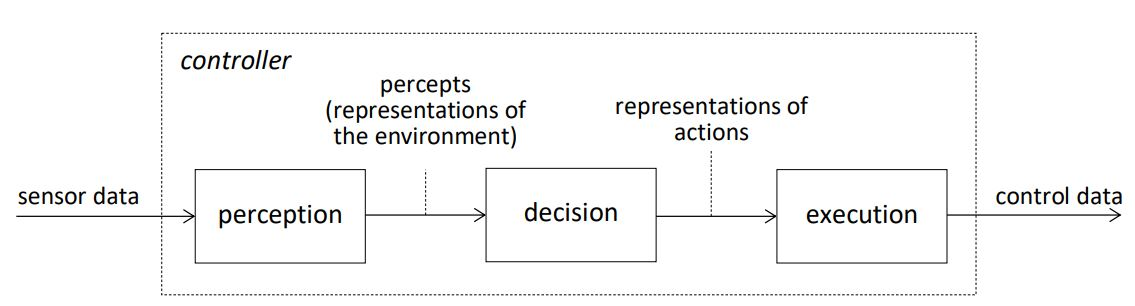
\includegraphics[height=4cm]{../arguments/decisionModule.JPG}
\end{center}
\subsection{Agent classification}
In view of our goals it is important to classify agents according to the complexity of their
decision-making function.\newline
\newline
A first distinction is between \textbf{reactive} and \textbf{proactive} agents. A purely
reactive agent is an agent that decides what to do only on the basis of the state of the perceived state of
its environment; in other words, such an agents simply reacts to elements of the current external (or
internal) situation. A proactive agent, on the contrary, is also sensitive to the future, at least as far as
this can be anticipated by the agent.\newline
\newline
Purely reactive agents are often further classified in the two categories of simple
reflex agent and model-based reflex agents, and proactive agents in the two categories of goal-based
agents and utility-based agents.
\subsubsection*{Simple reflex agents}
Simple reflex agents are agents whose decisions at time t are based on the agent’s
perceptions at time $t$.\newline
Simple reflex agents are stateless and therefore have no memory of past perceptions and
actions.
\subsubsection*{Model-based reflex agents}
Many types of behaviours cannot be implemented by a simple reflex agent, because
relevant information about the environment may not be currently accessible through the
agent’s sensors.\newline
Model-based reflex agents maintain a model that represents aspect of the environment
that are not currently accessible through the sensors.\newline
In any case, an agent of this type is still reflex, in the sense that its next action will be
completely determined by the current perceptions and the current model ot the
environment
\subsubsection*{Goal-based agents}
Reflex agents (either simple or model-based) are realised in such a way that they pursue
some fixed goal.\newline
A goal-based agent is an agent that can, within limits, select what goals to pursue and how
to pursue them.